\chapter{绪论}
\section{研究背景}
答辩是一种高密度的知识表达活动。参赛者不仅需要在有限时间内说明问题、方案、创新和验证，还需要根据评委追问迅速定位材料依据。实际准备往往以反复修改PPT和自行计时为主，难以回答三个关键问题：陈述是否覆盖材料中的关键结论，表达节奏在哪些时间点失衡，以及回答是否真正回应了问题。

通用对话模型可以给出润色建议，但直接把整篇材料交给模型仍存在上下文长度、证据定位和幻觉问题。检索增强生成通过先检索相关片段再生成回答，使输出可以绑定知识来源\cite{lewis2020rag}。移动终端又天然拥有摄像头、麦克风和振动能力，因此适合把“材料知识库、连续陈述、低干扰提醒、复盘报告和评委追问”组织为一个闭环。

本项目不依赖实验室、生物样本或专用传感器。用户只需自己的论文或演示材料和一部手机即可实践，这一边界与参赛团队的现实条件相符。系统也不承担教师管理、班级作业、社交或商业支付，避免把资源分散到与个人训练无关的功能。

\section{研究问题}
本文围绕四个工程问题展开。第一，如何让AI问题和内容评价受当前项目材料约束，并向用户展示证据片段。第二，如何在录制流畅性、端侧推理频率和隐私之间取得平衡。第三，如何用一套后端契约支撑Flutter与HarmonyOS原生客户端。第四，如何只评价可观察的表达行为，不越界推断情绪、性格、可信度或医学意义上的紧张程度。

\section{工作内容}
本文完成的工作包括：定义跨端统一的OpenAPI契约；实现Rust、Axum、SeaORM和SQLite后端；实现材料转换、OCR入口、分块、向量存储与项目内余弦检索；实现JWT账号体系与可撤销刷新令牌；实现训练会话、音频识别、五维报告和AI评委问答；实现Flutter客户端主流程；建立HarmonyOS 6原生Stage工程和C++端侧指标ABI；建立Docker Compose与Caddy部署方案；建立不允许虚构数据的测试和论文生产流程。

\section{论文结构}
第二章讨论公开资料和需求分析方法；第三章说明技术选型；第四至第七章分别介绍总体架构、数据接口、材料知识库和AI评委；第八至第十章讨论端侧AI及三端实现；第十一章说明隐私安全；第十二章说明部署运维；第十三、十四章给出测试与用户评估；第十五章为使用说明；最后给出结论与待完成事项。

\chapter{公开资料调研与需求分析}
\section{目标用户与使用情境}
目标用户是准备课程设计、毕业设计、创新创业或计算机应用竞赛答辩的大学生。典型情境是用户在宿舍、教室或安静公共空间独立练习，无法临时组织多名评委，也不希望原始训练视频长期上传。设备条件以普通手机和公网服务器为上限，不假设持续连接高性能工作站。

核心任务从用户视角表现为：建立一个答辩项目，导入自己已有的材料，确认系统成功提取内容，按真实时间完成连续陈述，查看有时间定位和材料证据的报告，随后进入评委模式回答不同类型的追问。历史趋势的价值在于比较同一项目多次训练，而不是把不同主题的绝对分数混为排名。

\section{竞品与方法边界}
公开可见的演讲训练产品常见能力包括计时、语速、口头禅、眼神或姿态提示；通用AI产品常见能力包括摘要、问答与文本评价。本项目的差异不在于声称单项算法首创，而在于把项目材料作为评价边界，将原始视频留在端侧，并在HarmonyOS 6上以原生能力完成适配验证。

对视觉分析必须设置边界。摄像头画面可以支持“是否出镜、面部是否大致朝向镜头、身体关键点是否稳定”等可观察指标，但不能可靠推出用户的性格、诚实程度或临床焦虑。系统文案、数据结构和模型输出都不包含这类标签。

\section{需求获取方案}
需求分析采用半结构访谈、任务观察和小规模可用性测试。计划邀请至少5名、目标8名近期有答辩经历的学生。访谈问题围绕当前练习方法、最难获得的反馈、是否接受音频临时上传、对材料证据的理解、报告阅读顺序和删除需求。每位参与者需要知情同意，可随时退出，记录时使用编号而非姓名。

\pending{尚未完成真实参与者招募。不得把计划人数写成样本量，也不得生成平均分、百分比或引语。访谈记录模板见附录。}

\section{功能需求}
功能需求分为账号、项目材料、训练、报告、评委问答和历史六组。账号支持用户名和密码注册登录；材料支持PDF、PPTX、DOCX、文本和图片，OCR文本可查看和纠正；训练支持前置摄像头、本地视频、计时和超时振动；报告固定包含内容、表达、时间、视觉和问答维度；问题覆盖技术、应用、创新、风险和质疑；删除项目时级联删除服务端材料、片段、报告和临时媒体。

\section{非功能需求}
五分钟训练应稳定录制，网络中断不丢失本地视频；报告目标是在训练完成后60秒内生成，但只有在供应商服务和网络满足条件时才验收。访问令牌有效期15分钟，刷新令牌有效期30天。端侧抽帧推理目标不低于5 FPS，同时不能明显影响录制。中文为默认界面语言，可保留必要英文术语。

\chapter{关键技术与选型}
\section{Flutter与原生能力}
Flutter以Dart统一iOS和Android界面，配合Riverpod管理状态、GoRouter管理路由、Dio管理HTTP请求。其优势是两端视觉和业务流程一致，且可通过插件调用AVFoundation与CameraX。Flutter官方文档给出了跨平台渲染、插件和构建机制\cite{flutter}。本项目不承诺App Store上架，iOS交付边界是开发调试签名；Android交付可安装APK。

\section{HarmonyOS 6原生实现}
HarmonyOS端采用Stage模型、ArkTS和ArkUI，不使用WebView封装。原生实现可以直接接入系统权限、CameraKit、AVRecorder、振动、通知、后台任务和本地关系型存储。官方开发文档是系统API版本适配的主要依据\cite{harmonydev}。工程把训练预览保留为XComponent surface，并通过N-API连接共享C++核心。

HarmonyOS适配的创新表述应保持可验证：它面向我国自主移动操作系统生态，降低产品对单一平台的依赖，验证核心AI能力在国产终端上的迁移、性能和隐私路径。本文不把操作系统或第三方框架的知识产权归属于项目团队。

\section{Rust后端}
Rust通过所有权和类型系统减少内存安全问题\cite{rustbook}。Axum建立在Tokio异步运行时和Tower服务抽象上\cite{axum}，适合实现JSON、multipart上传、中间件和结构化日志。SeaORM提供异步实体访问与迁移支持\cite{seaorm}。单机竞赛系统使用SQLite WAL可降低部署复杂度，并允许读操作与单个写事务并行\cite{sqlitewal}。

\section{检索增强与供应商抽象}
材料分块后调用兼容接口生成向量，向量以JSON数组保存在SQLite。检索时只读取当前项目的片段，在Rust进程内计算余弦相似度，避免引入独立向量数据库。对当前规模而言，这一实现易于备份和审计；若单项目片段达到数万级，才需要评估专用索引。

LLM、ASR和OCR通过环境变量配置兼容OpenAI协议的国产服务。未配置密钥时，健康检查返回AI未配置，相关接口返回明确服务不可用错误，不回退到伪造内容。这样可以区分“程序路径可用”和“真实模型结果已验证”。

\chapter{系统总体设计}
\section{设计原则}
系统遵循材料有界、视频本地、失败显式、指标可解释和三端一致五项原则。材料有界要求内容判断和评委问题只能引用当前项目片段；视频本地要求服务端API不存在视频上传入口；失败显式要求模型或供应商不可用时返回错误；指标可解释要求报告展示摘要、时间点和证据；三端一致要求字段和评分含义由OpenAPI与C++ ABI共同定义。

\section{逻辑架构}
系统分为移动客户端、API服务、任务处理与外部AI服务四层。客户端负责账号、材料选择、录制、本地保存、低频抽帧和报告展示。API服务负责鉴权、资源所有权检查、元数据读写和接口契约。任务处理器从数据库领取材料解析任务，调用LibreOffice、Poppler、OCR和嵌入接口。外部AI服务只接收完成特定任务所需的最小数据。

\begin{figure}[H]
\centering
\resizebox{\textwidth}{!}{\begin{tikzpicture}[node distance=1.8cm, every node/.style={draw,rounded corners=2pt,minimum height=1cm,align=center,font=\small},arrow/.style={->,thick,color=jade}]
\node (mobile) {Flutter客户端\\iOS / Android};
\node (harmony) [below of=mobile] {ArkUI客户端\\HarmonyOS 6};
\node (api) [right of=mobile,xshift=3.2cm,yshift=-0.9cm] {Axum API\\JWT与资源边界};
\node (db) [right of=api,xshift=3.2cm,yshift=0.9cm] {SQLite WAL\\业务数据与任务};
\node (worker) [right of=api,xshift=3.2cm,yshift=-0.9cm] {持久化Worker\\解析与报告};
\node (ai) [right of=worker,xshift=3.0cm] {国产AI服务\\LLM/ASR/OCR};
\draw[arrow] (mobile) -- (api); \draw[arrow] (harmony) -- (api);
\draw[arrow] (api) -- (db); \draw[arrow] (api) -- (worker);
\draw[arrow] (worker) -- (db); \draw[arrow] (worker) -- (ai);
\end{tikzpicture}}
\caption{SpeechMirror逻辑架构}
\end{figure}

\section{核心流程}
材料流程为上传、落盘、任务入队、文本提取、必要时OCR、分块、向量生成和状态回写。训练流程为创建会话、本地录制、端侧指标采样、音频临时上传、ASR、完成会话和报告生成。问答流程为检索材料、生成问题、保存证据、接收回答、再次检索并生成评价和追问。

\section{异常与恢复}
材料上传在返回前已经完成文件和数据库记录持久化。材料解析、训练ASR、回答ASR和报告生成统一进入数据库任务队列，保存queued、running、completed和failed状态及结构化结果；服务启动时把遗留running任务恢复为queued。worker失败后把错误写入任务，材料任务还同步更新材料状态。音频文件写入临时目录，在ASR成功或失败后主动删除，后台清理器每五分钟检查超过30分钟的遗留文件。

\chapter{数据模型与接口设计}
\section{实体关系}
核心实体包括用户、刷新令牌、项目、材料、材料片段、分析任务、训练会话、转写分段、端侧指标、训练报告、评委问题和用户回答。用户拥有项目和会话；项目级删除通过外键级联移除材料片段、会话、报告和问答记录，并另外删除文档文件。

\begin{longtable}{p{3.1cm}p{4.0cm}p{7.0cm}}
\caption{核心数据表及用途}\\
\toprule 表名 & 主键与关联 & 用途 \\
\midrule
\endfirsthead
\toprule 表名 & 主键与关联 & 用途 \\
\midrule
\endhead
users & id & 用户名、Argon2id密码摘要和创建时间 \\
\path{refresh_tokens} & \path{user_id} & 哈希后的刷新令牌、过期时间与撤销状态 \\
projects & user\_id & 项目名称、说明和目标答辩时长 \\
documents & project\_id & 文件路径、媒体类型、解析状态和纠正文本 \\
\path{document_chunks} & \path{document_id}, \path{project_id} & 片段序号、内容和可选向量 \\
\path{analysis_jobs} & \path{resource_id} & 持久化任务状态和错误 \\
\path{rehearsal_sessions} & \path{project_id}, \path{user_id} & 训练时长、转写和本地视频引用 \\
\path{session_metrics} & \path{session_id} & 时间戳、人脸、视线、姿态与音频电平 \\
reports & session\_id & 五维报告JSON \\
\path{jury_questions} & \path{project_id}, \path{session_id} & 问题类型、文本和材料证据 \\
\path{jury_answers} & \path{question_id}, \path{session_id} & 回答文本和评价JSON \\
\bottomrule
\end{longtable}

\section{认证与所有权}
密码采用Argon2id散列，相关算法建议见RFC 9106\cite{rfc9106}。访问令牌采用JWT，有效期15分钟，结构和校验遵循RFC 7519\cite{rfc7519}。刷新令牌为高熵随机值，服务端只保存SHA-256摘要；刷新时旧令牌立即撤销并轮换新令牌。每个受保护路由先解析访问令牌，再以user\_id过滤项目或训练会话，避免只凭UUID访问他人资源。

\section{OpenAPI契约}
契约位于仓库\texttt{openapi/openapi.yaml}，当前覆盖20条路径。Flutter请求层与ArkTS请求层使用相同字段名。上传采用multipart/form-data，其余写操作采用JSON。错误响应固定包含code和message，客户端不得通过解析自然语言判断错误类型。

\section{删除语义}
删除项目是彻底删除而非软删除：事务中的外键级联移除数据库记录，随后删除材料文件。原始视频从未进入服务端，需由客户端提供本地视频管理。若文件删除失败，服务端记录日志，运维清理任务应按无数据库引用的文件进行二次回收。

\chapter{材料解析与项目知识库}
\section{五类材料处理}
纯文本直接按UTF-8读取。PDF首先由pdftotext按布局提取；文本少于阈值时，把页面以160 DPI渲染为PNG后进入OCR。DOCX和PPTX先由LibreOffice无界面转换为PDF，再复用PDF流程。PNG和JPEG直接进入OCR。所有外部进程都检查退出状态并捕获标准错误。

\section{分块策略}
当前分块上限为800个Unicode字符，重叠100字符，并优先在句号、问号、感叹号或换行处截断。该策略保留段落语义并降低模型输入长度。每个片段保存document\_id、project\_id和ordinal，使检索结果既能回到原材料，也能保持原始顺序。

\section{OCR纠正}
OCR不可避免地受扫描质量、字体、表格和公式影响。客户端材料详情需要展示提取文本，并允许用户纠正；提交纠正后服务端先删除旧片段，再重新分块和生成向量。纠正入口比隐藏OCR错误更重要，因为后续问题和评价都依赖这份文本。

\section{检索与证据校验}
当AI供应商已配置时，查询和材料片段进入同一嵌入模型，Rust计算余弦相似度并选择前若干片段。未配置嵌入时只允许开发环境按原顺序读取片段，不能据此声称语义检索性能。生成提示要求模型返回chunk\_id和quote，服务端逐条确认引用编号属于当前检索集合，且引文是对应片段中的原文；没有有效证据时拒绝保存报告、问题或回答评价。

\chapter{AI评委与可解释报告}
\section{问题生成}
问题生成检索“项目背景、技术方案、创新点、实验结果、局限性和风险”等查询，要求模型生成技术、应用、创新、风险和质疑类别的问题。每个问题保存材料证据和可选session\_id。用户可以重建问题组，但历史回答不被新问题覆盖。

\section{连续追问}
回答评价同时输入原问题、用户回答和重新检索的材料。输出包括score、relevance、accuracy、evidence、suggestions和follow\_up。追问不是独立聊天话术，而应针对回答中未证实、含糊或遗漏的部分。任何“正确”判断都应能回到材料或明确标注材料不足。

\section{五维报告}
内容维度由材料约束的模型评价产生；表达维度使用语速和口头禅；时间维度比较目标与实际时长；视觉维度使用端侧结构化指标；问答维度在完成评委问答后更新。报告展示每一维摘要，内容维度展示证据，时间线展示可复盘事件。系统不把五维简单平均为单一人格化结论。

\section{语速与口头禅}
中文语速按去除空白后的字符数除以时长计算。当前舒适区间暂设为每分钟180至260字，用于提示而不是规范性判定。口头禅统计“然后、就是、那个、其实、嗯、啊”等词的直接出现次数。该词表需要在真实测试中检查误报，例如材料中作为技术术语或引用出现的情况。

\section{模型置信与失败}
模型返回的confidence仅表示本次内容评价响应的自报置信信息，不等于统计校准概率。供应商未配置、超时、返回非JSON或字段异常时，接口失败并保留本地媒体，不生成替代报告。Flutter训练页提供重试音频分析，避免网络错误导致视频丢失。

\chapter{端侧视觉指标设计}
\section{可观察指标}
端侧只输出face\_detected、gaze\_centered、posture\_score和confidence。face\_detected是布尔值，其余值限定在0至1。输出携带timestamp\_ms，与训练开始时刻对齐。服务端拒绝范围外数值，防止模型或桥接错误污染报告。

\section{共享C++ ABI}
C ABI比直接暴露C++类更适合跨Swift、Kotlin/JNI与ArkTS/N-API。接口包括ABI版本、创建、销毁、RGBA帧分析和最后错误。没有模型、输出数量不符或结果越界都返回明确枚举值。默认构建未启用MindSpore Lite时返回\path{MODEL_NOT_LOADED}，不产生占位指标。

\section{MindSpore Lite适配}
MindSpore Lite面向端侧推理\cite{mindsporelite}。适配层设置1至4个CPU线程，关闭默认FP16，要求输入为与采样帧尺寸一致的NHWC RGB张量，输出为四个归一化值。真实模型需要记录来源、授权、训练数据边界、输入尺寸、量化方式和指标解释。

\section{抽帧与性能预算}
录制与推理使用不同队列。摄像头保持正常录制帧率，分析只按目标5 FPS抽帧；若推理连续超预算，则降低分析频率而不阻塞编码。上传前可以按时间窗口聚合，避免每帧一个HTTP请求。性能验收记录设备型号、系统版本、环境温度、帧率、CPU占用、内存和十五分钟温升。

\pending{尚无合法模型文件和三端真机测量，不能报告5 FPS达成、准确率、温升或能耗对比。}

\chapter{Flutter客户端实现}
\section{应用结构}
Flutter工程由主题、模型、API客户端、认证控制器、路由和页面组成。Riverpod提供ApiClient与认证状态，GoRouter根据会话状态在登录页和项目页之间重定向。Dio集中处理基址、超时、Bearer头、401刷新和结构化错误。访问及刷新令牌使用flutter\_secure\_storage保存。

\section{项目与材料页面}
项目页支持创建项目并展示目标时长。详情页并行读取项目与材料列表，以processing、ready和failed区分处理状态；只有存在ready材料时才允许进入训练和评委。文件选择限制为PDF、PPTX、DOCX、TXT、Markdown、PNG和JPEG。

\section{训练页面}
训练页选择前置摄像头，摄像头录像关闭自带音轨，音频由独立录音器保存为M4A。停止时把摄像头临时视频复制到应用文档目录，然后只上传音频。达到目标时长时触发一次重振动。ASR或报告失败时页面显示本地视频路径和重试按钮。训练音频与评委回答音频使用不同接口，回答转写不会覆盖完整训练转写。

\section{报告与评委页面}
报告页展示语速、时长、口头禅、五维条形、材料引文、建议和时间定位。评委页可以生成问题、输入文本或录制语音回答，并展示相关性、准确性、建议和追问。视觉指标桥接尚未完成，因此Flutter当前不上传视觉样本；接口用null表示本维度不可评分，界面显示“—”并明确说明未采集，不把缺失数据画成零分。

\IfFileExists{figures/login_screen.png}{
\begin{figure}[H]\centering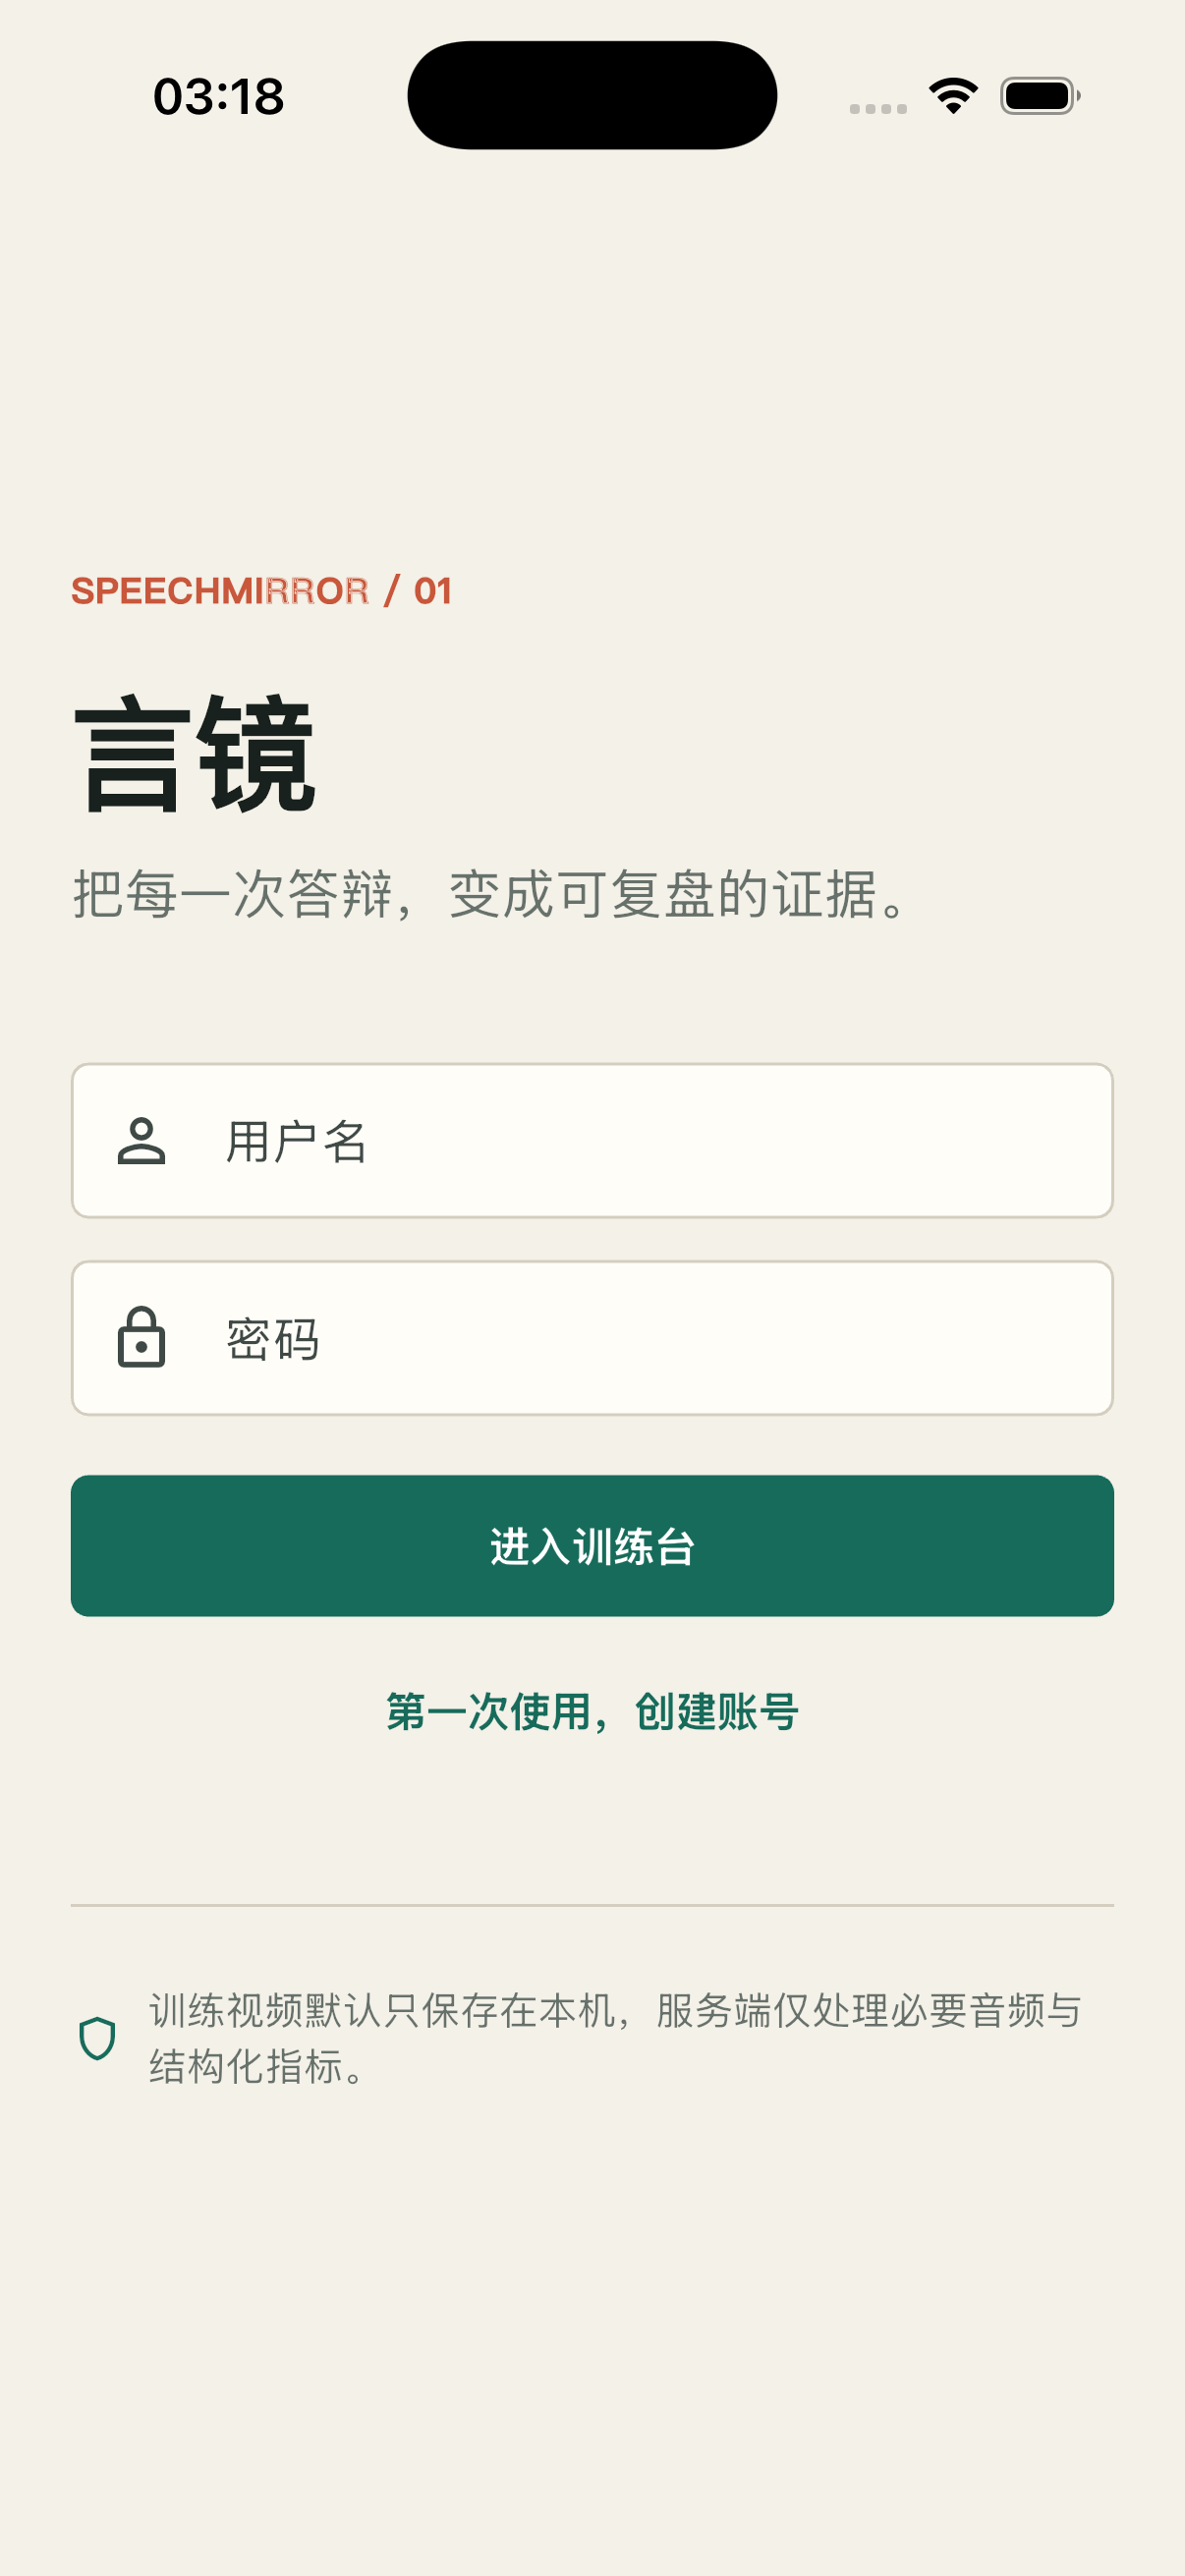
\includegraphics[width=0.46\textwidth]{figures/login_screen.png}\caption{iOS模拟器中的Flutter登录页实际运行截图}\end{figure}
}{\pending{Flutter登录页截图将在golden渲染完成后插入。}}

\chapter{HarmonyOS 6原生适配与创新}
\section{原生工程}
HarmonyOS工程包含AppScope、entry HAP、Stage EntryAbility、ArkUI页面、NetworkKit请求层和N-API模块。登录、项目、材料状态、训练、报告与评委页面沿用统一信息架构，但控件和生命周期由ArkUI原生实现，不嵌入Flutter或网页。

\section{系统能力协同}
训练页使用XComponent预留CameraKit surface，以Vibrator在超时时做低干扰提醒。后续真机实现将使用AVRecorder保存本地视频，后台任务只负责可恢复的上传或状态查询，不在后台持续打开摄像头。通知用于报告生成完成等异步事件，避免训练中持续弹出提示。

\section{隐私友好的端云协同}
姿态和视线特征在HarmonyOS设备上经N-API调用C++核心，只上传结构化结果。原始视频保留在应用沙箱。该路径展示了隐私边界可以作为跨端契约的一部分，而不只是隐私政策文本。服务端甚至不提供视频上传路由，从架构上减少误传可能。

\section{适配价值与限制}
HarmonyOS版本用于验证同一知识库、会话和报告在国产终端上的一致访问，并比较CPU推理、录制流畅度和能耗。创新点是原生适配、端云协同和可验证隐私路径的组合。当前工作站没有DevEco Studio与HarmonyOS 6 SDK，工程尚未生成HAP，CameraKit与AVRecorder也未绑定实际设备profile。

\pending{需要HarmonyOS 6真机完成安装、权限、录制、N-API加载、MindSpore推理、后台任务、通知、弱网和能耗测试。}

\chapter{隐私、安全与伦理边界}
\section{数据最小化}
系统收集实现功能所需的最小数据。账号不要求真实姓名和手机号；视频默认不上传；音频只为ASR临时传输；视觉上传的是数值指标；报告保留转写和材料引用以供复盘。个人信息处理应遵循目的明确、最小必要和公开透明原则\cite{pipl}。

\section{传输与存储}
公网部署由Caddy自动提供HTTPS。密码只保存Argon2id摘要，刷新令牌只保存哈希。SQLite、材料与日志使用持久卷，备份文件应加密并限制访问。日志不记录Authorization头、音频正文、完整转写或AI密钥。生产环境必须替换开发JWT密钥。

\section{提示注入与材料污染}
用户材料可能包含“忽略此前要求”等指令性文本。材料在系统中是待评价的数据而非系统指令，提示模板要明确这一层级。引用必须检查chunk\_id，输出展示引文而不是只展示模型总结。对上传文件还应限制尺寸、类型、转换超时和解析进程权限。

\section{评价伦理}
系统只评价可观察行为和材料覆盖，不评价情绪、人格、可信度、心理疾病或就业能力。分数不是排名，也不是教师成绩。模型置信不应被包装为科学测量。用户可以删除项目及其服务端派生数据，本地视频由用户自行管理。

\chapter{部署与运维}
\section{容器部署}
后端Docker镜像采用Rust构建阶段和Debian运行阶段。运行镜像安装LibreOffice、Poppler、Noto CJK字体和CA证书，以非root用户启动。Compose只包含API与Caddy，不引入Redis；SQLite、材料和Caddy证书使用命名卷。

\section{配置管理}
环境变量包括\path{BIND_ADDR}、\path{DATABASE_URL}、\path{STORAGE_DIR}、\path{JWT_SECRET}、\path{CORS_ALLOWED_ORIGINS}、\path{AI_BASE_URL}、\path{AI_API_KEY}、各模型名和外部程序路径。\texttt{.env}被Git忽略，仓库只提供\texttt{.env.example}。浏览器跨域访问默认关闭，只能按明确的HTTPS来源白名单开启；移动端通过编译参数设置API基址，生产环境只使用HTTPS。

\section{日志与健康检查}
Tracing输出结构化请求日志，健康接口返回\path{status}和\path{ai_configured}。健康检查不调用付费模型，也不泄露模型密钥。建议进一步增加数据库可写、磁盘剩余空间、队列积压和供应商延迟指标，并设置日志轮换。

\section{备份恢复}
备份SQLite时应使用在线备份API或在短暂停写窗口复制数据库及WAL相关文件，不能只复制主文件。材料卷与数据库快照需要同一恢复点。恢复演练应检查用户登录、材料状态、报告读取和新任务领取。

\chapter{软件测试与当前结果}
\section{测试策略}
测试分为单元、接口集成、组件、构建、真机回归和非功能测试。单元测试覆盖分块、口头禅统计和材料引文强校验；接口测试覆盖注册、JWT轮换、项目创建和CORS白名单；Flutter测试覆盖报告模型解析；C++测试覆盖ABI和未加载模型的失败路径。构建验证用于证明产物可生成，但不代替设备运行。

\section{已执行结果}
\begin{table}[H]
\centering
\caption{截至2026年9月25日的真实执行结果}
\begin{tabularx}{\textwidth}{p{4.0cm}p{5.0cm}X}
\toprule 对象 & 命令 & 结果 \\
\midrule
Rust API & \texttt{cargo test} & 6项测试通过，0失败，含引文与令牌轮换校验 \\
本地HTTP & \texttt{curl}真实请求 & 健康、注册、项目创建、Markdown上传及ready状态通过 \\
任务队列 & 本地可控响应存根 & 回答ASR、训练ASR和报告任务完成；存根结果不计为业务结论 \\
Flutter & \texttt{flutter analyze} & 0项问题 \\
Flutter & \texttt{flutter test} & 1项测试通过，0失败 \\
Android & \texttt{flutter build apk --debug} & 成功生成调试APK，约163 MB \\
iOS & \texttt{flutter build ios --simulator} & 模拟器构建、安装和登录页启动通过 \\
C++核心 & \texttt{cmake; ctest} & 1项ABI契约测试通过 \\
OpenAPI & Ruby YAML解析 & 3.1.0文档可解析，共20条路径 \\
\bottomrule
\end{tabularx}
\end{table}

\section{待执行测试}
需要在配置真实供应商后验证PDF、扫描PDF、PPTX、DOCX、文本和图片的解析；完成五分钟音频ASR并测量报告生成时间；检查问题引用是否属于材料；在Android和iOS真机验证断网保留视频；在HarmonyOS 6真机验证媒体与N-API；执行项目删除后的数据库和文件检查。

\section{验收判定}
测试报告必须保存日期、提交版本、设备、系统、网络、输入材料和原始日志。性能指标报告中同时给出中位数、范围和样本数。失败用例不能从统计中静默删除。任何截图都应遮蔽账号、令牌、密钥和个人材料。

\chapter{用户评估方案}
\section{参与者与任务}
目标邀请8名近期参与过答辩的学生，最低有效样本5名。每人完成注册、创建项目、上传一份材料、确认提取文本、完成一次三分钟训练、阅读报告、回答两个问题和删除测试项目。研究者只在参与者无法继续时提供预先定义的提示。

\section{度量方法}
记录任务成功率、完成时间、错误点、求助次数和主观反馈。可使用SUS量表作为整体可用性参考\cite{brooke1996sus}，但小样本只作描述性分析，不夸大统计推断。启发式检查参考一致性、错误预防、状态可见和用户控制等原则\cite{nielsen1994}。

\section{访谈提纲}
访谈询问：报告首先关注哪个部分；材料证据是否增加信任；哪些提示会干扰陈述；能否理解视频本地与音频临时上传的差别；视觉指标是否容易被误解；删除入口是否足够清楚；与现有练习方式相比是否愿意再次使用。

\section{数据真实性}
每份记录使用P01至P08编号，保留原始时间戳和问题版本。报告表由两位作者交叉核对。未回答项目标为缺失，不以平均值填补。参与者引语在去标识后使用，任何尚未收集的字段保持空白。

\pending{本章当前只描述方案。真实参与者、SUS得分、任务成功率和引语尚未产生。}

\chapter{系统使用说明}
\section{部署服务端}
在VPS安装Docker与Compose，复制环境变量样例，生成至少32字节随机JWT密钥，填写域名和AI供应商凭据。运行\texttt{docker compose up -d --build}，确认Caddy证书成功、健康接口为ok且ai\_configured为true。定期备份数据卷。

\section{安装移动端}
Android使用生成的APK调试安装；正式演示前应生成签名release APK并记录SHA-256。iOS通过Xcode和现有开发者签名安装到测试设备，不承诺App Store发布。HarmonyOS使用DevEco Studio配置签名并安装HAP，必须记录SDK和设备版本。

\section{创建项目与材料}
登录后新建项目，设置名称、说明和目标时长。上传材料后等待状态变为“已完成解析”。扫描文件应打开提取文本检查错字；若关键信息错误，先纠正再训练。材料状态失败时查看错误，不应继续生成问题。

\section{完成一次训练}
将手机置于稳定位置，使头肩位于引导区域。开始后界面只保留当前时长、目标时长和画面位置提示；达到目标时间系统振动一次。结束后视频保存本地，音频上传进行转写。网络失败可重试分析，不要删除本地媒体。

\section{阅读报告与问答}
先看时间和表达等确定性指标，再看内容摘要和材料引文。对不符合材料的结论应记录并反馈。进入评委席后按真实答辩方式回答，优先说明结论、依据和局限。追问用于发现薄弱点，不代表正式比赛题目。

\chapter{结论与后续工作}
本文给出了SpeechMirror从需求边界、数据模型、接口、材料知识库、AI评委、端侧指标到三端客户端和部署的工程实现。系统把材料证据与报告绑定，把视频上传从服务端能力中移除，并把HarmonyOS 6作为原生迁移与隐私验证平台。当前Rust、Flutter、Android构建和C++契约已通过本地验证。

项目仍有四项决定最终结论的工作：配置并验证真实国产AI供应商；接入合法MindSpore Lite模型；在iOS、Android和HarmonyOS 6真机完成媒体与性能测试；完成至少5人的真实访谈和可用性任务。只有这些数据到位后，论文才能扩展到95至105页并形成竞赛终稿。后续还应增加ASR分段时间戳、断点续传、加密备份和自动化隐私回归测试。
